\documentclass[aspectratio=169,12pt]{beamer}
\usepackage{amsmath}
\usepackage{amssymb}
\usepackage[most]{tcolorbox}
\usepackage{tikz}
\usepackage{graphicx}
\usepackage[sfdefault,lf]{FiraSans}
\renewcommand{\familydefault}{\sfdefault}
\setlength{\parindent}{0pt}
\everymath{\displaystyle}

\setbeamertemplate{navigation symbols}{}
\setbeamertemplate{footline}{}
\setbeamertemplate{headline}{}

\definecolor{mmpageWhite}{HTML}{FCFBF7}
\definecolor{mmtanSoft}{HTML}{F7F5EF}
\definecolor{mmgreenDeep}{HTML}{244B2C}
\definecolor{mmgreenLeaf}{HTML}{5D8A56}
\definecolor{mmgreenSoft}{HTML}{E4EFD9}
\definecolor{mmtext}{HTML}{163221}

\setbeamercolor{background canvas}{bg=mmpageWhite}
\setbeamercolor{normal text}{fg=mmtext,bg=mmpageWhite}

\newtcolorbox{MMProblemCard}[1][]{enhanced,breakable=false,colback=white,colframe=black,boxrule=1.5pt,arc=8pt,left=5pt,right=5pt,top=4pt,bottom=4pt,before skip=0pt,after skip=0pt,height=0.245\textheight,valign=top,#1}
\newcommand{\KoruIcon}{\raisebox{-0.2em}{
\includegraphics[height=1.05em]{../../SITE/header-logo.png}}}
\newcommand{\ScaffoldIcons}[1]{\ifcase#1\or \KoruIcon\or \KoruIcon\hspace{0.22em}\KoruIcon\or \KoruIcon\hspace{0.22em}\KoruIcon\hspace{0.22em}\KoruIcon\fi}
\newcommand{\WorksheetTitle}[2]{%
  {\colorbox{mmtanSoft}{\parbox[c][2.0em][c]{0.975\linewidth}{%
    \hspace{0.25em}{\Large\bfseries\textcolor{mmgreenDeep}{#1}\hfill\ScaffoldIcons{#2}}}}
  \par\vspace{0.08em}{\color{mmgreenLeaf}\rule{\linewidth}{2.0pt}}\par\vspace{0.04em}}
}
\newcommand{\MMProblem}[2]{\begin{MMProblemCard}\raggedright\small\textbf{#1.} #2\par\end{MMProblemCard}}

\setbeamertemplate{background}{
 \begin{tikzpicture}[remember picture,overlay]
 \draw[black,line width=1.5pt,rounded corners=10pt]
 ([xshift=0.45cm,yshift=-0.45cm]current page.north west)
 rectangle
 ([xshift=-0.45cm,yshift=0.45cm]current page.south east);
 \end{tikzpicture}
}

% Default worksheet generation rules:
% use notes-style beamer pages
% use bordered cards for individual problems
% target 9 problems per frame in a 3x3 grid
% target 3 frames per scaffold by default where content allows

\begin{document}\begin{frame}[t]
\WorksheetTitle{Build Tasks}
\vspace{-0.18em}
\begin{columns}[T,onlytextwidth]
\begin{column}{0.32\textwidth}\MMProblem{1}{Find the area.\\[0.4em]
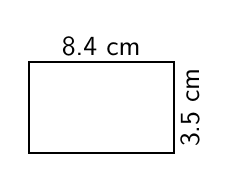
\begin{tikzpicture}[x=0.23cm,y=0.23cm,baseline=(current bounding box.center)]
  \draw[thick] (0,0) rectangle (8,5);
  \node at (4,5.9) {8.4 cm};
  \node[rotate=90] at (8.9,2.5) {3.5 cm};
\end{tikzpicture}}\end{column}
\begin{column}{0.32\textwidth}\MMProblem{2}{Find the area.\\[0.4em]
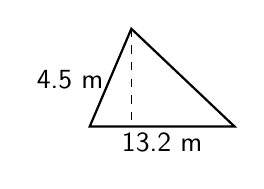
\begin{tikzpicture}[x=0.23cm,y=0.23cm,baseline=(current bounding box.center)]
  \coordinate (A) at (0,0);
  \coordinate (B) at (8,0);
  \coordinate (C) at (2.3,5.4);
  \draw[thick] (A)--(B)--(C)--cycle;
  \draw[dashed] (C)--(2.3,0);
  \node at (4,-0.9) {13.2 m};
  \node at (1.3,2.6) [left] {4.5 m};
\end{tikzpicture}}\end{column}
\begin{column}{0.32\textwidth}\MMProblem{3}{Find the area.\\[0.4em]
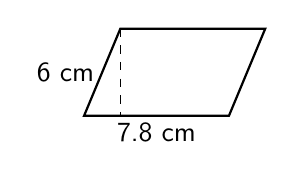
\begin{tikzpicture}[x=0.23cm,y=0.23cm,baseline=(current bounding box.center)]
  \coordinate (A) at (0,0);
  \coordinate (B) at (8,0);
  \coordinate (C) at (10,4.8);
  \coordinate (D) at (2,4.8);
  \draw[thick] (A)--(B)--(C)--(D)--cycle;
  \draw[dashed] (D)--(2,0);
  \node at (4,-0.9) {7.8 cm};
  \node at (1.1,2.4) [left] {6 cm};
\end{tikzpicture}}\end{column}
\end{columns}
\vspace{0.45em}
\begin{columns}[T,onlytextwidth]
\begin{column}{0.32\textwidth}\MMProblem{4}{Find the area.\\[0.4em]
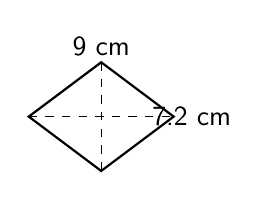
\begin{tikzpicture}[x=0.23cm,y=0.23cm,baseline=(current bounding box.center)]
  \coordinate (T) at (4,6);
  \coordinate (R) at (8,3);
  \coordinate (B) at (4,0);
  \coordinate (L) at (0,3);
  \draw[thick] (T)--(R)--(B)--(L)--cycle;
  \draw[dashed] (T)--(B);
  \draw[dashed] (L)--(R);
  \node at (4,6.9) {9 cm};
  \node at (9.0,3) {7.2 cm};
\end{tikzpicture}}\end{column}
\begin{column}{0.32\textwidth}\MMProblem{5}{Find the area.\\[0.4em]
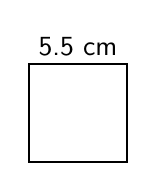
\begin{tikzpicture}[x=0.25cm,y=0.25cm,baseline=(current bounding box.center)]
  \draw[thick] (0,0) rectangle (5,5);
  \node at (2.5,5.9) {5.5 cm};
\end{tikzpicture}}\end{column}
\begin{column}{0.32\textwidth}\MMProblem{6}{A rectangle is 16 cm by 9 cm. Find its area.}\end{column}
\end{columns}
\vspace{0.45em}
\begin{columns}[T,onlytextwidth]
\begin{column}{0.32\textwidth}\MMProblem{7}{A triangle has base 15 m and height 8 m. Find its area.}\end{column}
\begin{column}{0.32\textwidth}\MMProblem{8}{A parallelogram has base 12.5 cm and height 7 cm. Find its area.}\end{column}
\begin{column}{0.32\textwidth}\MMProblem{9}{A kite has diagonals 14 cm and 11 cm. Find its area.}\end{column}
\end{columns}
\end{frame}
\begin{frame}[t]
\WorksheetTitle{Build Tasks}
\vspace{-0.18em}
\begin{columns}[T,onlytextwidth]
\begin{column}{0.32\textwidth}\MMProblem{1}{The area of a rectangle is 54 cm\mbox{$^2$}. Its width is 6 cm. Find the length.}\end{column}
\begin{column}{0.32\textwidth}\MMProblem{2}{The area of a triangle is 36 m\mbox{$^2$}. Its base is 9 m. Find the height.}\end{column}
\begin{column}{0.32\textwidth}\MMProblem{3}{The area of a parallelogram is 63 cm\mbox{$^2$}. Its height is 7 cm. Find the base.}\end{column}
\end{columns}
\vspace{0.45em}
\begin{columns}[T,onlytextwidth]
\begin{column}{0.32\textwidth}\MMProblem{4}{The area of a kite is 48 cm\mbox{$^2$}. One diagonal is 12 cm. Find the other diagonal.}\end{column}
\begin{column}{0.32\textwidth}\MMProblem{5}{A square has area 81 cm\mbox{$^2$}. Find the side length.}\end{column}
\begin{column}{0.32\textwidth}\MMProblem{6}{Which has the greater area: a rectangle \mbox{$9$} cm by \mbox{$6$} cm or a triangle with base \mbox{$14$} cm and height \mbox{$8$} cm?}\end{column}
\end{columns}
\vspace{0.45em}
\begin{columns}[T,onlytextwidth]
\begin{column}{0.32\textwidth}\MMProblem{7}{A triangle and a parallelogram both have base 10 cm and height 6 cm. Which has the greater area, and by how much?}\end{column}
\begin{column}{0.32\textwidth}\MMProblem{8}{Explain why a triangle with the same base and height as a rectangle has half the area.}\end{column}
\begin{column}{0.32\textwidth}\MMProblem{9}{}\end{column}
\end{columns}
\end{frame}
\end{document}
